
%(BEGIN_QUESTION)
% Copyright 2015, Tony R. Kuphaldt, released under the Creative Commons Attribution License (v 1.0)
% This means you may do almost anything with this work of mine, so long as you give me proper credit

Examine this overcurrent protection system for a feeder, supplying three-phase power to a set of industrial loads from a substation bus:

$$\includegraphics[width=15.5cm]{i02562x01.eps}$$

Explain why 50/51 overcurrent protection is necessary at all, since each of the loads has its own set of fuses to protect against overcurrent conditions.

\vskip 10pt

Suppose the cable connecting phase 2 CT to the 50-2/51-2 relay fails shorted, such that the relay no longer senses current through that phase.  Will the other two overcurrent relays continue to provide adequate protection?  Explain why or why not, in detail.

\vfil 
\underbar{file i02562}
\eject
%(END_QUESTION)





%(BEGIN_ANSWER)

This is a graded question -- no answers or hints given!

%(END_ANSWER)





%(BEGIN_NOTES)

While each set of three fuses provides overcurrent protection for their respective loads, the 50/51 relays provide overcurrent protection for the {\it feeder} and for the {\it circuit breaker} (52), should there ever be a fault in one of those.  You may imagine a phase-to-phase or phase-to-ground short-circuit occuring at some point along the feeder conductors, which lies ``upstream'' of the fuses: none of that fault current would pass through any of those fuses, and so none of the fuses provide protection against that location and type of fault.

\vskip 10pt

Failure of the 50-2/51-2 relay means that overcurrent conditions in phase 2 would not be detected, or acted upon.  So long as the other two relays were perfectly functional, the breaker and feeder would still be protected against overcurrent events involving one of the other (non-faulted) phases.  Any phase-to-phase fault, for example, would still be detected and the circuit breaker opened as a result, because any current passing through phase 2 would also pass through at least one of the other phases as part of a complete circuit.

However, neither the 50-1/51-1 or 50-3/51-3 relays would protect against a phase-to-ground fault on phase 2 f the feeder, or phase 2 within the circuit breaker.  Thus, an important aspect of this system's protection would be defeated by the CT cable failure on phase 2.

%INDEX% Protective relay: instantaneous overcurrent (50)
%INDEX% Protective relay: time-overcurrent (51)

%(END_NOTES)


